\section{Performancevergleich mit anderen Algorithmen}\label{chap:Performance}

In der Metaheuristik existieren eine Vielzahl evolutionärer Algorithmen (EAs)\nomenclature{EAs}{evolutionäre Algorithmen}. Alle basieren auf der biologischen Evolution und/oder dem sozialen Verhalten einer Spezies und ermöglichen es komplexe Optimierungsprobleme zu lösen, welche zum Teil mit herkömmlichen Methoden nicht lösbar sind. \newline
In dem vorliegenden Dashboard wurde der ACO Algorithmus verschiedenen weiteren EA Algorithmen im Hinblick auf die Qualität der Ergebnisse gegenübergestellt. \newline 
Alle Algorithmen lösen dabei ein Minimierungsproblem auf entweder der Himmelblau- oder der Rosenbrockfunktion. Es werden ausschließlich zwei Parameter (x1, x2), sowie ein diskreter Zahlenraum betrachtet.\newline 
Der Zahlenraum (untere und obere Grenze), sowie die Anzahl an Evolutionen und die Populationsgröße können konfiguriert werden, um die Auswirkung der verschiedenen Parameter auf die Ergebnisse der Algorithmen zu sehen. \newline 
Folgende Algorithmen werden im Dashboard gegenübergestellt: 
\begin{itemize}
    \item Ant Colony Optimization Algorithm
    \item Ant Lion Optimization Algorithm 
    \item Bat Optimization Algorithm 
    \item Cat Swarm Optimization Algorithm
    \item Dragonfly Optimization Algorithm 
    \item Firefly Optimization Algorithm 
\end{itemize}
Der oder die am besten abschneidenden Algorithmen werden nach Abschluss der Berechnung grün, der am schlechtesten abschneidene Algorithmus rot und die Anderen gelb hervorgehoben.
\begin{figure}[H]
 \centering
 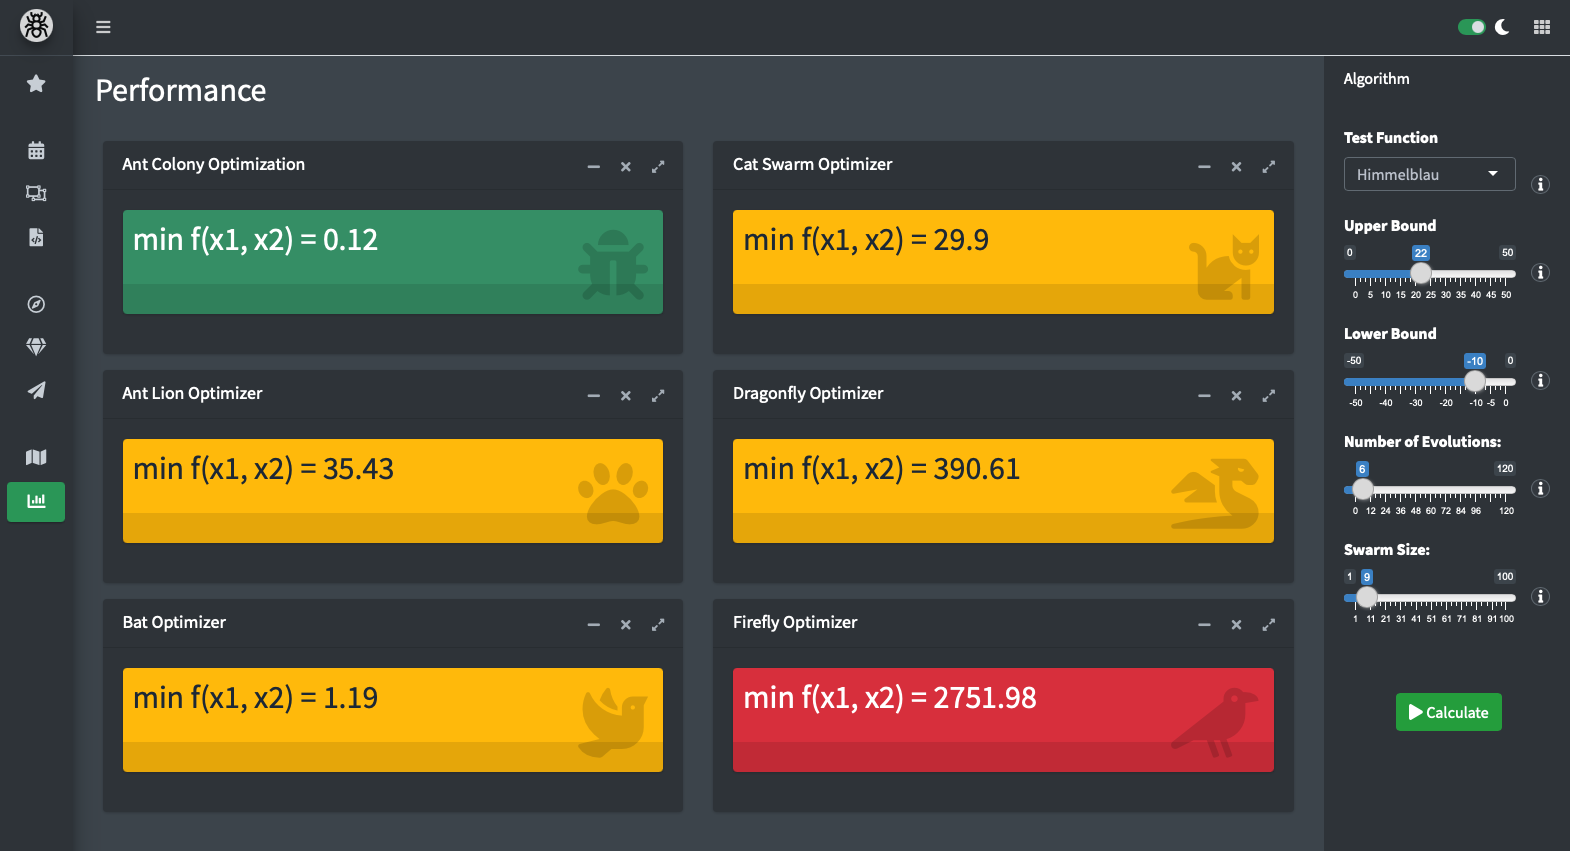
\includegraphics[scale=0.2]{"images/06_Performancevergleich/performance_tab.png"}
 \caption{Performance Tab mit farblicher Hervorhebung der Ergebnisse der einzelnen Algorithmen}
 \label{fig:performance_tab}
\end{figure}

Die Implementation der einzelnen EA Algorithmen, mit Ausnahme des ACO Algorithmus basieren auf dem Paket \emph{metaheuristicOpt} \citep{Riza2019}. Ein Paket, welches verschiedenste metaheuristische Optimierungsalgorithmen implementiert. \newline 
Die Implementation des ACO Algorithmus basiert auf dem Paket evoper \cite{Garcia2018}.
Der Performance Tab ist wie folgt designed: Er besteht aus sechs bs4Dash Karten, welche selber nochmal valueBoxen enthalten. Diese valueBoxen werden vom Server aus befüllt. Dabei sind Informationen, wie das Icon oder der erste Teil des Headers statisch, die Color Property und der zweite Teil des Headers dynamisch. \newline 
Die Controlbar, welche die Input Elemente zum Konfigurieren der Algorithmen enthält ist nicht in dem mod\_performance\_tab.R Modul, sondern in der fct\_update\_controlbar.R Datei enthalten. Diese Funktion updated den Inhalt der Controlbar abhängig von gerade ausgewählten Tab und muss folglich global und nicht in einem Modul implementiert sein. \newline 

\begin{figure}[h]
 \centering
 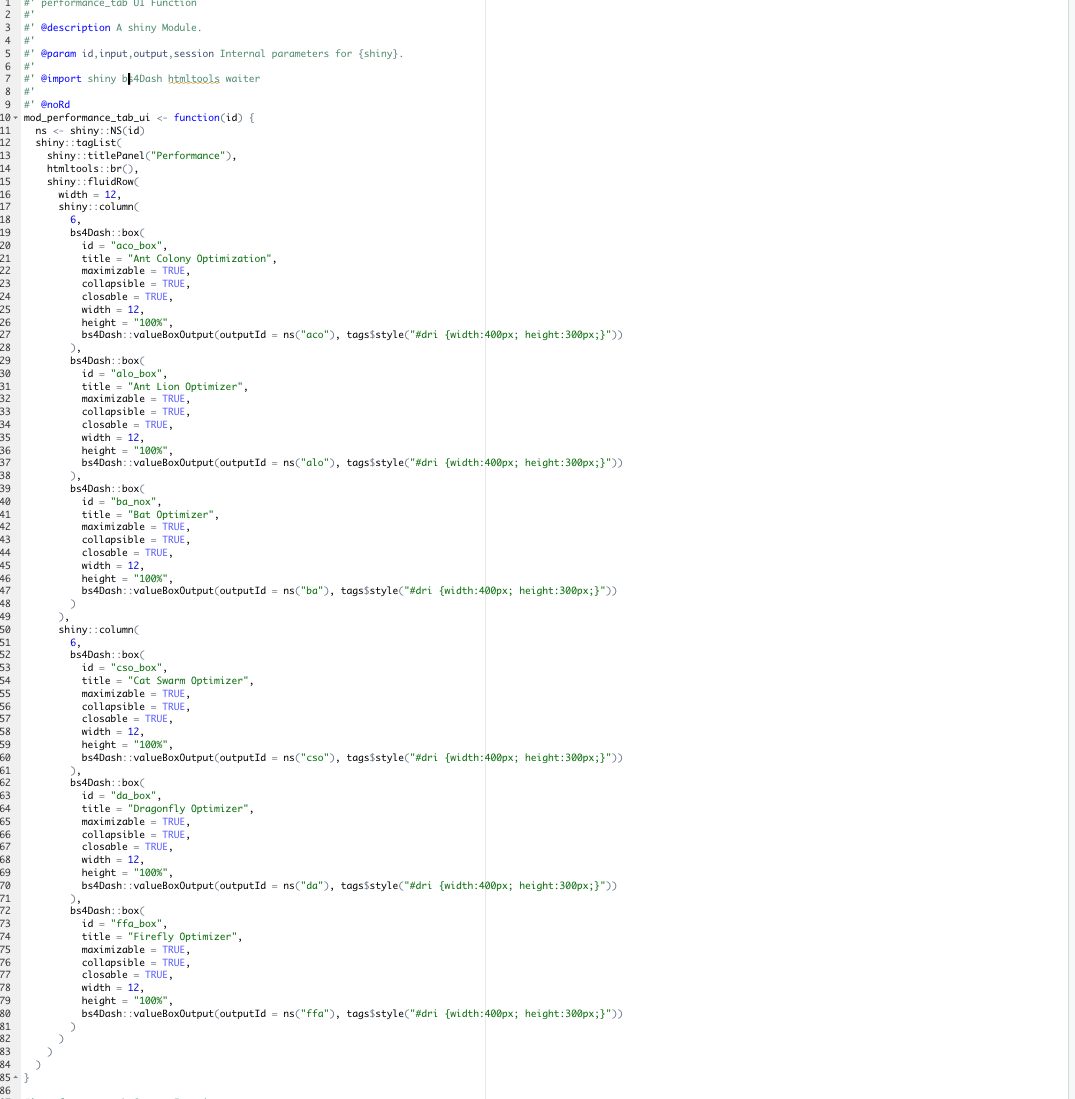
\includegraphics[scale=0.4]{"images/06_Performancevergleich/ui_performance_tab.png"}
 \caption{UI Funktion des Performance Tabs}
 \label{fig:ui_performance_tab}
\end{figure}

\begin{figure}[H]
 \centering
 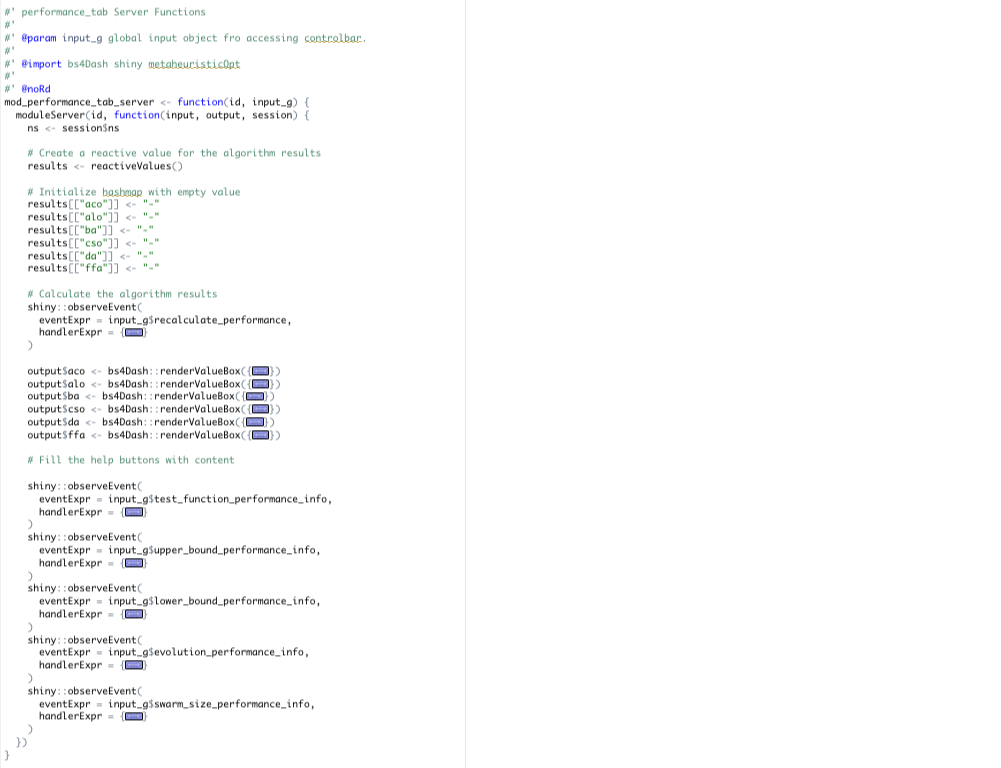
\includegraphics[scale=0.4]{"images/06_Performancevergleich/server_performance_tab.png"}
 \caption{Server Funktion des Performance Tabs mit eingeklappten Funktionen}
 \label{fig:server_performance_tab}
\end{figure}

Abschließend gilt es die get\_color Funktion zu erwähnen. Diese updated die valueBox Farbe, abhängig vom Ergebnis des Algorithmus. Die Logik basiert dabei auf der Idee, dass die Mimima der Rosenbrock- und Himmelblau Funktion jeweils bei y=0 liegen. Umso dichter also die in die Kostenfunktion eingesetzten Funktionswerte an Null sind, umso besser perfomt der Algorithmus. 
\begin{figure}[H]
 \centering
 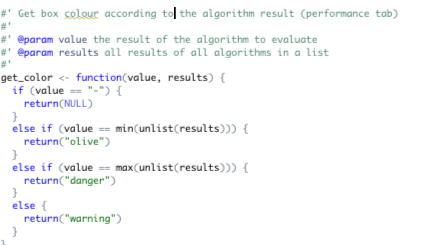
\includegraphics[scale=0.4]{"images/06_Performancevergleich/utils_get_color.png"}
 \caption{get\_color Funktion, welche die Box-Farbe abhängig vom Ergebnis des Algorithmus updated}
 \label{fig:server_performance_tab}
\end{figure}